\chapter{Revisão Inicial}

\section{Arquitetura x Organização}
\textbf{Arquitetura de computadores} se refere a atributos do sistema que são visíveis ao programador (Assembly).

\underline{Exemplos:} conjunto de instruçoes, endereçamento de memória, ...

\textbf{Organização de computadores} está relacionado às unidades operacionais do computador e suas interconexões (barramentos).\\[0.2cm]

\underline{Exemplos:} sinais de controle, tecnologia de memória e cache, ...



\section{Execução de Programas}
A execução de programas envolve a execução de instruções. No início do ciclo de instrução, o processador busca da memória a instrução cujo endereço está no \textbf{program counter (PC)}. A instrução é carregada no \textbf{registrador de instrução} (instruction register - IR) e  o processador finalmente decodifica a instrução para sua futura execução.

A instrução decodificada pode ser de diferentes \textbf{tipos}:

\begin{itemize}
  \item Transferência de dados entre processador e memória (LOAD e STORE);
  \item Transferência de dados entre periféricos e processador (\textit{input} e \textit{output});
  \item Execução de operações lógicas e aritméticas;
  \item Alterações na sequência de execução das instruções (\textit{branches}).
\end{itemize}

O \textbf{ciclo de instruções} envolve as seguintes etapas:

\begin{itemize}
  \item \textbf{Instruction Address Calculation (IAC):} determinação do endereço da próxima instrução;
  \item \textbf{Instruction Fetch (IF):} carregamento da instrução no processador;
  \item \textbf{Instruction Decoding (ID):} determinação do tipo de instrução e seus operandos necessários;
  \item \textbf{Operand Fetch (OF):} busca dos operandos;
  \item \textbf{Data Operation (DO):} execução da operação;
  \item \textbf{Operand Store (OS):} escrita do resultado da operação.
\end{itemize}

\subsection{Desvios}
No caso de uma execução sequencial, o endereço da próxima instrução é obtido através de uma operação de soma no PC. Entretanto, as execuções de programas raramente são sequenciais, onde em alguns pontos do código caminhos alternativos são tomados. Blocos de decisão e \textit{loops} são responsáveis por tais desvios, presentes em linguagens de alto nível. Nas instruções de máquina essas operações são implementadas por \textit{branches} e \textit{jumps}.





\section{Pipelining}
Pipelining é a forma de executar múltiplas instruções, de forma sobreposta, acelerando a execução de uma programa como um todo (e não executar instruções mais rapidamente).

As instruções são executadas de forma sobreposta, divida por estágios, que devem ser completados em um ciclo de \textit{clock}. Qualquer combinação de estágios deve poder ocorrer ao mesmo tempo. Entretanto, tal fato acaba resultando em um desbalanceamento entre os estágios, dado que alguns estágios são mais lentos que outros, limitando o desempenho. Um exemplo, são estágios de execução (EX) com operações de ponto flutuante, que demoram mais que um ciclo.

Alguns estágios dependem da saída de estágios anteriores. Assim, \textit{overheads} são postos por registradores de pipeline, chamados de \textbf{latches}. Os dados e controles necessários por estágios avançados são passados através dos \textit{latches}, adiantando a passagem destes parâmetros.



\subsubsection*{Instruction Fetch}
\textbf{Busca a instrução da memória e carrega do \textit{registrador de instrução}}. A posição da instrução é determinada pelo \texttt{PC}. Ao fim do carregamento, o \texttt{PC} é incrementado em 4, determinando o endereço da próxima instrução (se não houver \textit{branch}), porém este é inserido no \texttt{NPC}. Logo a sequência acaba sendo:

\texttt{IR $\leftarrow$ Mem[PC]}

\texttt{NPC $\leftarrow$ PC + 4}




\subsubsection*{Instruction Decode}
\textbf{Decodifica a instrução no IR e acessa os registradores indicados na mesma.} O registradores fazem parte de um conjunto de registradores de uso do programador e são carregados para registradores temporários para uso na instrução (chamamos eles de \texttt{A} e \texttt{B}).

Os 16 bits menos significativos do \texttt{IR} são armazenados no registrador de imediato, o \texttt{Imm}. A decodificação e busca de operando é feita em parelelo, chamada de \textit{decodificação de campo fixo}.



\subsubsection*{Execution}
\textbf{Executa as operações indicadas na instrução.} Esta depende da instrução, podendo ser:
\begin{itemize}
  \item \textbf{Referência a memória}, onde o efetivo é calculado com a ajuda do imediato: \texttt{ALUOutput $\leftarrow$ A + Imm};

  \item \textbf{ALU registrador-registrador}, que são operações aritméticas envolvendo registradores apenas: \texttt{ALUOutput $\leftarrow$ A func B};

  \item \textbf{ALU registrador-memória}, que são operações  aritméticas envolvendo a memória e um registrador: \texttt{ALUOutput $\leftarrow$ A op Imm}

  \item \textbf{Branches}, que são desvios condicionais no fluxo de execução do código:

  \texttt{ALUOutput $\leftarrow$ NPC + Imm}

  \texttt{Cond $\leftarrow$ (A op 0)}
\end{itemize}



\subsubsection*{Acesso à memória}
\textbf{Executa \texttt{loads}, \texttt{stores} e \textit{branches}.} Se a instrução for \texttt{LOAD}, o dado é lido da memória e colocado em um registrador próprio, o \texttt{LMD}.

\texttt{LMD $\leftarrow$ Mem[ALUOutput]}

Se for um \texttt{STORE}, os dados contidos no registrador indicado são escritos em memória.

\texttt{Mem[ALUOutput] $\leftarrow$ B}

Se for um \textit{branch}, o \texttt{PC} ganha um valor diferente dependendo da tomada de decisão na condição. Logo:

\texttt{if (cond)}\\
\texttt{PC $\leftarrow$ ALUOutput}\\
\texttt{else}\\
\texttt{PC $\leftarrow$ NPC}\\



\subsubsection*{Write Back}
\textbf{Escreve os resultados das operações nos registradores e/ou memória.} Logo envolve instruções dos tipos:

\begin{itemize}
  \item \textbf{ALU registrador-registrador:} \texttt{Regs[IR16\dots 20] $\leftarrow$ ALUOutput};

  \item \textbf{ALU registrador-imediato:} \texttt{Regs[IR11\dots 15] $\leftarrow$ ALUOutput};

  \item \textbf{Load}: \texttt{Regs[IR11\dots 15] $\leftarrow$ LMD}.
\end{itemize}




\subsection{Hazards}
Situações que impedem que o próximo estágio da instrução seja executado no próximo ciclo de clock, sendo a maior fonte de atraso no pipeline, deixando-o ocioso.

\textbf{\textit{Stall}}: nome do atraso resultante de um hazard

\textbf{\textit{Bubble}}: atraso a nível de estágio



\subsubsection{Hazard Estrutural}
Para executar instruções de forma paralela as unidades funcionais devem estar sobrepostas (\textit{pipelined}) e duplicadas. \textbf{Quando instruções não podem ser executadas em paralelo por falta de recurso} (\textit{hardware}), temos um hazard estrutural. Logo, ocorrem por dois motivos:

\begin{enumerate}
  \item As unidades funcionais não estão dispostas de maneira sobreposta;

  \item Os recursos não estão replicados suficientemente, levando a conflitos de utilização.
\end{enumerate}

As vezes vale a pena permitir um hazard estrutural pois o \textit{stall} pode ser menos custoso que um \textit{overhead} de paralelização ou inserção de mais \textit{hardware}




\subsubsection{Hazard de Dados}
Ocorrem quando o \textit{pipeline} para porque uma instrução precisa esperar o término de outra, o que chamamos de \textbf{dependência entre instruções}. Ocorre pois o \textit{pipeline} pode mudar a ordem acesso aos operando. Temos três tipos de dependências:

\begin{itemize}
  \item \textbf{\textsc{RAW} - Read After Write}: queremos ler um valor que ainda vamos escrever;

  \item \textbf{\textsc{WAW} - Write After Write}: queremos escrever um valor onde ainda precisamos escrever outro;

  \item \textbf{\textsc{WAR} - Write After Read}: queremos escrever um valor onde ainda precisamos ler outro;
\end{itemize}

Podemos tentar resolver com \textbf{\textit{forwarding}} (ou \textit{bypassing}): transferimos o dado necessário diretamente da unidade que o produz para a unidade que o necessita. Feitor por meio de ligação física direta.

\begin{figure}
  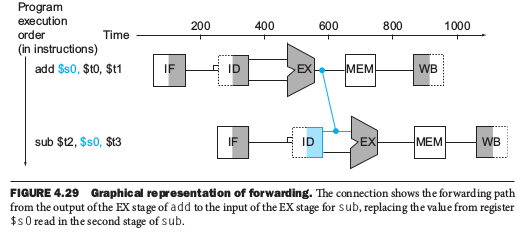
\includegraphics[width=\textwidth]{branch-forwarding}
  \label{fig:branch-forwarding}
  \caption{Esquema de Branch Forwarding}
\end{figure}

Algumas instruções, como o \texttt{LOAD}, apenas disponibilizam o dado em um estágio muito avançado, atrasando o \textit{pipeline} ao ponto de uma instrução seguinte. O \textbf{pipeline interlock} é o \textit{hardware} que detecta tal hazard e insere \textit{bubbles} o suficiente até que o \textit{forwarding} possa ser realizado corretamente e a execução continue.

\begin{figure}
  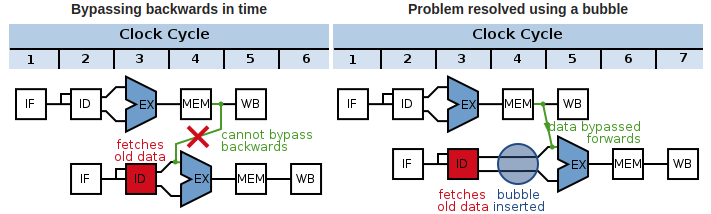
\includegraphics[width=\textwidth]{pipeline-interlock}
  \label{fig:pipeline-interlock}
  \caption{Inserção de \textit{bubbles} para acontecer o \textit{forwarding}}
\end{figure}

O compilador também pode auxiliar, identificando e evitando certos padrões, reeordenando o código de forma a evitar os \textit{stalls}. Chamamos isso de \textbf{pipeline scheduling}, onde o programa é separado em os blocos básicos e as instruções são escalonadas dentro deles.

\textbf{Blocos Básicos:} sequência de instruções onde não há desvios ou I/O. Todas as instruções são executadas se a primeira for.




\subsubsection{Hazard de Controle}
Define-se como \textbf{o atraso resultante da espera de saber se um desvio é tomado}. A instrução de desvio pode mudar o \texttt{PC} (\textit{branch taken}) ou não (\textit{not taken}) e, se tomado, este resultado só será conhecido no estágio \textsc{Mem}. Podemos reduzir combinando a previsão de tomada do desvio e cálculo prévio do novo do \texttt{PC}.

\textsc{Previsão Not Taken}\\
Todos os \textit{branchs} são tratados como \textit{not taken} e o \textit{pipeline} é carregado com as instruções seguintes a ele. O estado da máquina não é alterado até o desvio ser conhecido e se a previsão falhar, as mudanças são desfeitas, o que chamamos de \textbf{back out}.

\textsc{Previsão Taken}\\
Todos os \textit{branchs} são tratados como \textit{not taken} e o \textit{pipeline} é carregado com as instruções a partir do endereço apontado por ele. Não é muito efetiva, já que em várias arquiteturas ainda não se conhece o alvo do desvio.

\textsc{Delayed Branch}\\
Muito usado nos primeiros RISCs. O compilador tenta inserir um conjunto de instruções que sempre será executado após o \textit{branch}, independente do seu resultado. Chamamos este conjunto de \textbf{\textit{branch delay slot}}, o qual estará sempre após a instrução de desvio e normalmente tem tamanho 1. Há três formas de se escalonar:

\begin{itemize}
  \item \textbf{From before:} retira instruções \underline{independentes do desvio e posteriores a ele}, inserindo-as no \textit{slot}. Esta é a melhor opção e deve sempre ser tomada quando possível;

  \item \textbf{From target:} usado quando há maior probabilidade de \underline{desvio \textit{taken}}. Insere no \textit{slots} as instruções presentes no endereço do desvio. Se a previsão falhar, haverá trabalho disperdiçado;

  \item \textbf{From fall through:} usando quando há maior probabilidade de \underline{desvio \textit{not taken}}. Insere no \textit{slot} as instruções logo depois da instrução do desvio.
\end{itemize}

\begin{figure}
  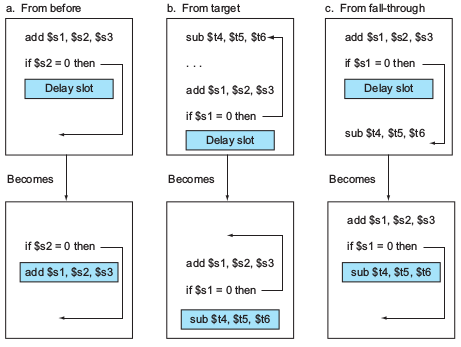
\includegraphics[width=\textwidth]{delayed-branch-scheme}
  \label{fig:delayed-branch-scheme}
  \caption{Escalonamentos do delayed branch}
\end{figure}

Se a previsão é correta, o \textit{delay slot} é executado. Caso contrário, fazemos o \textbf{cancelamento do \textit{branch}}: inserimos um \texttt{NOP} no \textit{delay slot} e executamos. Isso remove restrições extras a serem colocadas no \textit{slot}. Normalmente, os \textit{cancelling branches} são tomados quando há o \textit{not taken}.

Esta técnica possui limitações. Em tempo de compilação, é difícil de prever se vai haver o desvio e o conjunto de instruções podem conter outras depêndencias e \textit{branches} que impedem a previsão.




\section{Barramento}
\textsc{Definição:} meio de transmissão compartilhado que conecta dispositivos. Sua velocidade máxima é limitada pelo seu tamanho e o número de dispositivos conectados a ele.

Barramentos do tipo CPU-Memória são pequenos e de alta velocidade, enquanto os de I/O são maiores, acomodando diversos tipos de dispositivos, seguindo um determinado padrão.

Um barramento é composto por:

\begin{itemize}
  \item \textbf{Linhas de dados:} cada linha transporta 1 bit por vez;

  \item \textbf{Linhas de endereço:} onde o endereço da palavra acessada é colocado

  \item \textbf{Linhas de controle:} controlam o uso das linhas
    \begin{itemize}
      \item Memory write \& memory read
      \item Transfer ACK
      \item Bus request, que pede o controle do barramento
      \item Bus grant, que obtém o controle do barramento
      \item Clock e reset
    \end{itemize}
\end{itemize}

\begin{figure}
  \centering
  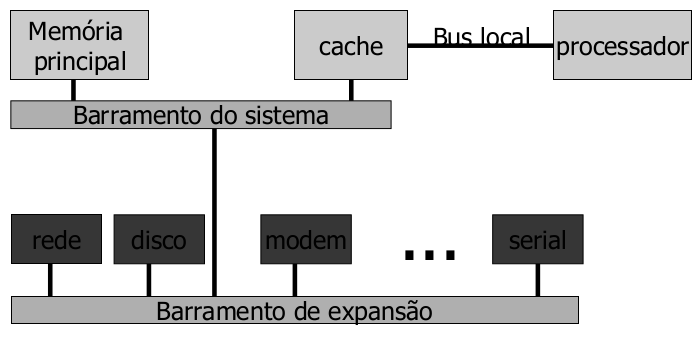
\includegraphics[width=0.8\textwidth]{buses-arch}
  \label{fig:buses-arch}
  \caption{Arquitetura com diferentes barramentos}
\end{figure}

A \textbf{leitura de dados da memória} é feita com o envio de um endereço e sinais de controle indicativo leitura. A memória coloca o dado no barramento e retira - ou \textit{deasserts} - o sinal de espera (\textit{wait}).

A \textbf{escrita dos dados em memória} é feita com a CPU enviando o endereço e do dado ao barramento. A memória retira estes sinais e atualiza o dado. Geralmente, a CPU não espera a confirmação.

Os \textbf{bus masters} são dispositivos que podem iniciar transações no barramento, como a CPU. Sistemas com vários masters necessitam de um esquema de arbitragem para resolução de conflitos, geralmente usando prioridade fixa ou randômica.


\textbf{Split transaction buses} são buses \textit{pipelined} ou \textit{packet-switched}. As transações no barramento são divididas em etapas, de forma a não bloquear o mesmo durante toda a transação. A unidade envolvida participa da arbitragem. As transações possuem \textit{tags}, para serem identificadas.

\underline{Exemplo:} transação de \textit{read} pode ser dividida em \textit{read-request} e \textit{memory-reply}.



\subsection{Síncronos x Assíncronos}
Nos \textbf{barramentos síncronos} uma das linhas de controle é um \textit{clock}. Os protocols para endereço e dados são fixos e baseados neste \textit{clock}. Normalmente são os barramentos CPU-Memória, uma vez que são rápidos e baratos. Devidos as distorções no \textit{clock} (\textit{clock skew}), eles não podem ser longos.

Já \textbf{barramentos assíncronos} usam protocolos de \textit{handshaking} entre o emissor e receptor do dado, provando um \textit{overhead} de sincronização a cada transação. Por isso são mais lentos, mas permitem que mais tipos de dispositivos sejam utilizados, sendo ótimos para gerênciar \textit{buses} de I/O.
